\documentclass{beamer}
\usepackage{amsmath}
\usepackage{amsfonts}
\usepackage{amssymb}
\usepackage{setspace}
\usepackage[utf8]{inputenc}
\usepackage[german]{babel}
\usepackage{algpseudocode}
%\usetheme{Madrid}Goettingen  Marburg   
%\usetheme{Amsterdam}
\usetheme{Madrid}

% theme
\usetheme{default}
\usecolortheme{default}
\usefonttheme{professionalfonts}

\setbeamertemplate{mini frames}[box]
\setbeamertemplate{navigation symbols}{}
\setbeamertemplate{itemize items}[default]
\setbeamertemplate{enumerate items}[default]
\setbeamercovered{highly dynamic}


%für zitat
\usepackage{microtype}
\usepackage{mdframed}

%caption next to figure
\usepackage{floatrow}
\usepackage{graphicx}

%text in ecke
\usepackage{eso-pic}

%figure in frame
\usepackage{capt-of}

%aufzählung
%\usepackage{enumitem}


\title[Intruder-Problem mit Potentialvergabe]{Optimierung des Intruder-Problems durch Potentialvergabe}
\author{Jens Harder}
\date{9. November 2015}

%definition zitat
\mdfdefinestyle{zitat}{
	hidealllines=true,leftline=true,linewidth=1.5pt,
	leftmargin=2.0em,innerleftmargin=1.0em,rightmargin=3.0em,
	innerrightmargin=0pt,innerbottommargin=0.5em, innertopmargin=0.5em}

\newtheorem{counter}{Theorem}
\newtheorem{mydef}[counter]{Definition}
%\newtheorem{theorem}[counter]{Theorem}
%\newtheorem{lemma}[counter]{Lemma}

%LineComment (pseudo)
\algnewcommand{\LineComment}[1]{\begingroup
	\setlength\parindent{0pt}\par\leftskip1.6em\rightskip3\leftskip /* #1 */ \par
	\endgroup}


\begin{document}
	
	\spacing{1.3}
	
	\begin{frame}
		\titlepage
	\end{frame}
	
	\begin{frame}
		\frametitle{Inhaltsverzeichnis}
		\large
		
		\tableofcontents
	\end{frame}
	
	\section{Das Intruder-Problem auf einem Baum}
	\begin{frame}
		\frametitle{Das Intruder-Problem auf einem Baum}
		\large
		\begin{itemize}
			\item Gesucht wird ein Eindringling
			
			\item Minimale Anzahl an Agenten
			
			\item Systematisches Absuchen des Baumes
			
			\item wichtige Eigenschaft: Monotonie

		\end{itemize}
	\end{frame}
		
%	\begin{frame}
%		\frametitle{Monotonie}
%		\large
%		
%		\begin{mydef}\label{def_monotonie}
%			Eine Strategie ist monoton, wenn sichergestellt wird, dass ein bereits dekontaminierter Knoten bis zur vollständigen Dekontaminierung des gesamten Graphen nicht erneut kontaminiert wird.
%		\end{mydef}
%%		\textbf{"'Eine Strategie ist monoton, wenn sichergestellt wird, dass ein bereits
%%			dekontaminierter Knoten bis zur vollständigen Dekontaminierung des gesamten Graphen nicht erneut kontaminiert wird."'}
%	\end{frame}
	
	{% Ab hier wird das Bild Hintergrundfüllend eingefügt
		\setbeamertemplate{background canvas}{
			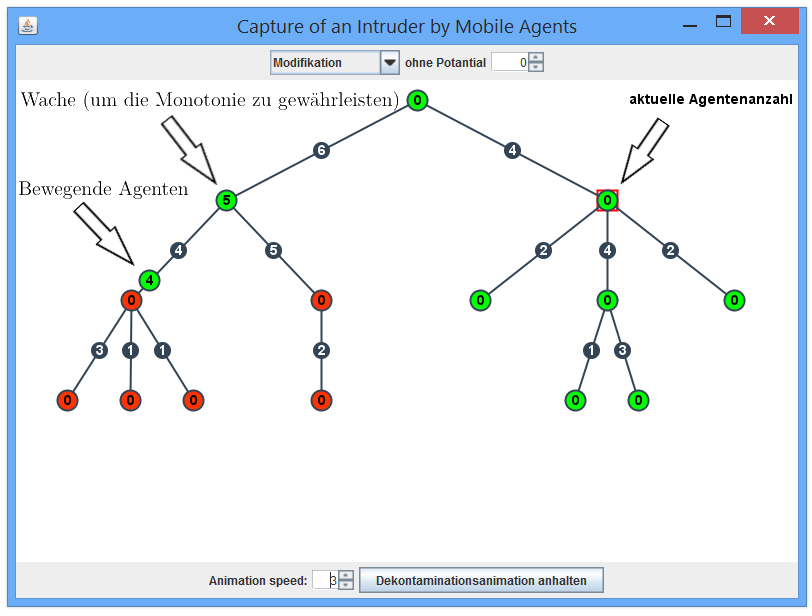
\includegraphics[%
			width=\paperwidth,
			height=\paperheight]{bilder/abb_erklaerung4.png}
		}
		\begin{frame}[plain]
			
%			\AddToShipoutPictureFG*{
%				\AtPageUpperLeft{\put(247,-40){\makebox[\paperwidth][l]{\cite{bildWahnbachtalsperre}}}}
%			}%
			
		\end{frame}
	}% hier ended die Gültigkeit des Bildeinfügens
	

	\section{Ziele der Bachelorarbeit}
	\begin{frame}
		\frametitle{Ziele der Bachelorarbeit}
		\large
		
		\begin{itemize}
			\item Modifikation des ursprünglichen Algorithmus\\
				(\textsc{Barriére} et al. (2002): Capture of an Intruder by Mobile Agents.)
			
			\item Algorithmus mit Potentialvergabe
			
			\begin{itemize}
				\item $k = 1$ auf einer Kante
				
				\item $k \geq 1$ auf einer Kante
				
				\item $k > 1$ auf mehrere Kanten verteilt
			\end{itemize}
			
			\item Implementierung der Algorithmen
			
		\end{itemize}
		
	\end{frame}
	
	\section{Nachrichtenberechnung}
	
		\begin{frame}
			\frametitle{Nachrichtenberechnung}
			\large

			
			\begin{itemize}
				
				\item $\omega(e) \geq 1$ ist das Kantengewicht einer Kante $e$
								
				\item $\omega(x) = \max_{e} \omega(e)$ für jede zu $x$ inzidente Kante $e$. Dann ist $\omega(x)$ das Knotengewicht des Knoten $x$
				
				\item $\mu(x)$ ist die minimale Anzahl an Agenten, die man für den Baum braucht, wenn man von diesem Knoten aus startet
				
				\item $\lambda_{y}(e)$  ist der Nachrichtenwert, der über Kante $e$ zu Knoten $y$ geschickt wird
				
			\end{itemize}
			
		\end{frame}
	
%	\begin{frame}
%		\frametitle{Nachrichtenberechnung in 3 Fällen}
%		\large
%		
%		1. Fall: Blattknoten ($\lambda_{y} = \omega(x)$)
%		
%		\centering
%		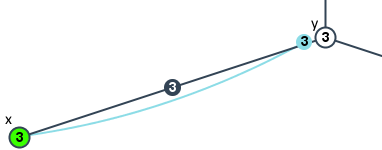
\includegraphics[width=.8\textwidth]{bilder/abb_blattknoten_NEU2.png}
%		\captionof{figure}{Das Knotengewicht des Blattknotens $x$ (grün) bestimmt den Wert Nachricht $\lambda_{y} = 3$ (blau) zum Nachbarknoten $y$.}
%		
%	\end{frame}
%	\begin{frame}
%		\frametitle{Nachrichtenberechnung in 3 Fällen}
%		\large
%		
%		2. Fall: $n-1$ empfangene Nachrichten ($\lambda_{y} = max\{l_{1},  l_{2} + \omega(x)\}$)
%		
%		\centering
%		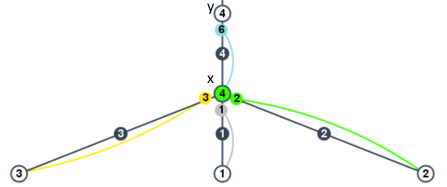
\includegraphics[width=.8\textwidth]{bilder/abb_paper_n-1knoten_NEU2.png}
%		\captionof{figure}{Der Wert der neuen Nachricht $\lambda_{y}$(blau) von Knoten $x$ zu Knoten $y$ beträgt 6, da $l_{2} + \omega(x) = 6$ (grün) größer ist als $l_{1} = 3$ (gelb).}
%		
%	\end{frame}
%	\begin{frame}
%		\frametitle{Nachrichtenberechnung in 3 Fällen}
%		\large
%		
%		3. Fall: $n$ empfangene Nachrichten ($\lambda_{y} = max\{l_{1},  l_{2} + \omega(x)\}$)
%		
%		\centering
%		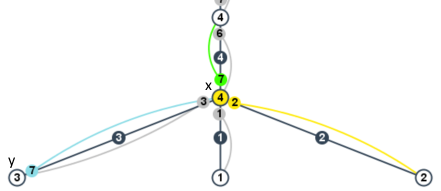
\includegraphics[width=.8\textwidth]{bilder/abb_paper_nknoten_NEU2.png}
%		\captionof{figure}{Die neue Nachricht $\lambda_{y}$ (blau) von Knoten $x$ zu Knoten y hat den Wert 7, da $l_{1} = 7$ (grün) größer ist als $l_{2} + \omega(x) = 6$ (gelb). Die Nachricht von $y$ zu $x$ (mit dem Wert = 3) wird bei dieser Berechnung ignoriert.}
%		
%	\end{frame}
%	
%	\begin{frame}
%		\frametitle{Berechnung der minimalen Agentenzahl}
%		\large
%		
%		\begin{itemize}
%			\item Berechne $\mu(x)$ für jeden Knoten $x$: $\mu(x) = max\{l_{1},  l_{2} + \omega(x)\}$
%			
%			\item Durchlauf durch alle Knoten, um das minimale $\mu$ zu finden
%			
%			\item Knoten $x$ mit minimalem $\mu$ ist die neue Homebase
%		\end{itemize}
%
%		
%	\end{frame}
%	
%	\begin{frame}
%		\frametitle{Wofür brauchen wir die Modifikation?}
%		\large
%
%		\begin{columns}[T] % align columns
%			\begin{column}{.5\textwidth}
%				\centering
%				\textbf{Ohne Modifikation}
%				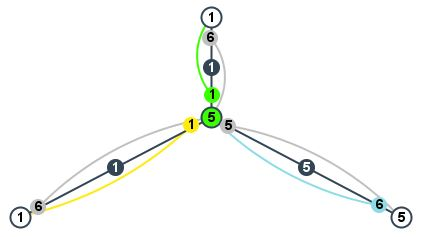
\includegraphics[width=\textwidth]{bilder/modifikation_ohne.jpg}
%				\captionof{figure}{Berechnung der Nachrichten mit dem ursprünglichen Algorithmus.}
%			\end{column}%
%			\hfill%
%			\begin{column}{.5\textwidth}
%				\centering
%				\textbf{Mit Modifikation}
%				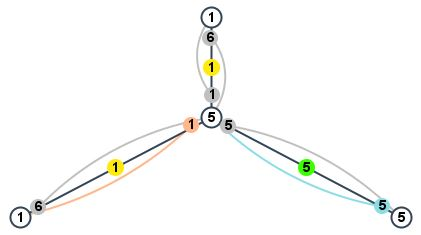
\includegraphics[width=\textwidth]{bilder/modifikation_mit.jpg}
%				\captionof{figure}{Berechnung der Nachrichten mit der modifizierten Variante.}
%			\end{column}
%		\end{columns}
%	\end{frame}
	
		
	\begin{frame}
		\frametitle{Modifizierte Nachrichtenberechnung}
		\large
		
		$\lambda_{y} = edge_{1} + edge_{2}$
		
		\centering
		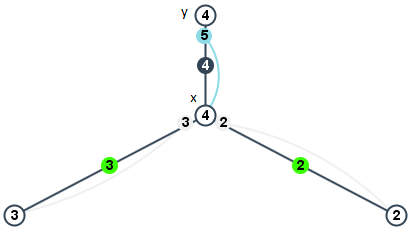
\includegraphics[width=.75\textwidth]{bilder/abb_neu_max1max2.png}
		\captionof{figure}{Die Nachricht $\lambda_{y}$ (blau) von x zu y hat den Wert 5, da $edge_{1} $ und $edge_{2}$ (beide grün) die entscheidenden Kanten sind.}
		
	\end{frame}
		
	\begin{frame}
		\frametitle{Modifizierte Nachrichtenberechnung}
		\large
		
		$\lambda_{y} = \max\{\lambda_{y}, \omega(x)\}$
		
		\centering
		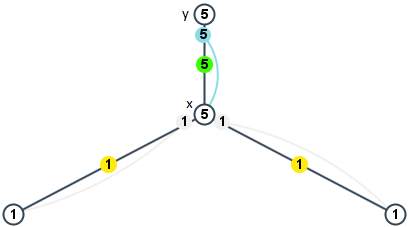
\includegraphics[width=.75\textwidth]{bilder/abb_neu_edge.png}
		\captionof{figure}{Da das Knotengewicht durch die Kante zwischen x und y bestimmt wird (grün), und dieses größer ist als die Summe der beiden normalen Kanten $edge_{1}$ und $edge_{2}$ (gelb), bestimmt diese Kante den Wert der Nachricht $\lambda_{y} = 5$ (blau).}
		
	\end{frame}
	
	\begin{frame}
		\frametitle{Modifizierte Nachrichtenberechnung}
		\large
		
		$\lambda_{y} = \max\{\lambda_{y}, l_{1}\}$
		
		\centering
		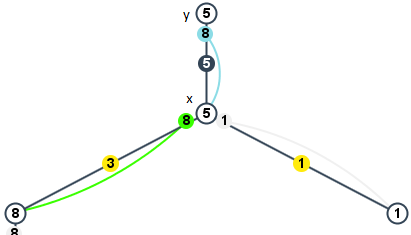
\includegraphics[width=.75\textwidth]{bilder/abb_neu_msgData.png}
		\captionof{figure}{Die größte Nachricht (grün), die an $x$ ankommt, ist größer als die bisher berechnete Nachricht und bestimmt daher den Nachrichtenwert $\lambda_{y} = 8$ (blau).}
		
	\end{frame}
	
	\begin{frame}
		\frametitle{Berechnung der minimalen Agentenzahl}
		\large
		
		\begin{itemize}
			\item Berechne $\mu(x)$ für jeden Knoten $x$: $\mu(x) = max\{edge_{1} + edge_{2},  l_{1}\}$
			
			\item Durchlauf durch alle Knoten, um das minimale $\mu$ zu finden
			
			\item Knoten $x$ mit minimalem $\mu$ ist die neue Homebase
		\end{itemize}
		
		
	\end{frame}

	
	\section{Das Potential-Problem}
	\begin{frame}
		\frametitle{Das Potential-Problem}
		\large
		
		\begin{itemize}
			\item Reduziere Kante(n) mit einem Potential $k$
			
			\item Kann das Potential immer sinnvoll angewendet werden?
			
			\item Auf welche Kanten soll das Potential angewendet werden
			
			\item Algorithmus
			
		\end{itemize}
		
	\end{frame}
	
	\subsection{Potential-Problem $k=1$}
	\begin{frame}
		\frametitle{Das Potential-Problem $k = 1$}
		\large
		
		\begin{itemize}
			\item Idee: Protokolliere die Kanten, von denen der Nachrichtenwert abhängt
			
			\item 3 Fälle, von denen die Nachrichten abhängen können:
			
				\large
				\begin{enumerate}[a)]
					
					\item $\lambda_{y} \gets edge_{1} + edge_{2}$   (aus den beiden größten Kanten)
					\label{potk=1_a}
					
					\item $\lambda_{y} \gets \omega(x)$   (aus der Kante, über welche die Nachricht gerade verschickt wird (diese entspricht dem Knotengewicht))
					\label{potk=1_b}
					
					\item $\lambda_{y} \gets l_{1}$   (aus der größten angekommenen Nachricht)
					\label{potk=1_c}
					
				\end{enumerate}
		\end{itemize}
	\end{frame}
	
	\begin{frame}
		\frametitle{Das Potential-Problem $k=1$}
		\large
		
		\begin{itemize}
			\item Fall \ref{potk=1_a}: $\lambda_{y} \gets edge_{1} + edge_{2}$
			
			\normalsize
			\item [ ]
			\item [ ]
				\begin{algorithmic}
					\If {$edge_{1} == edge_{3}$}
					\LineComment{(mindestens) drei gleich große Kanten}
					\State protokolliere: "`flag"'
%					\\
					\ElsIf {$edge_{2} == edge_{3}$}
					\LineComment{maximale Kante ist eindeutig}
					\State protokolliere: $edge_{1}$
%					\\
					\Else
					\LineComment{größte und zweitgrößte Kante ist eindeutig}
					\State protokolliere: $edge_{1}$ und $edge_{2}$
					\EndIf
				\end{algorithmic}
			
		\end{itemize}
				
	\end{frame}
	
	\begin{frame}
		\frametitle{Das Potential-Problem $k=1$}
		\large
		
		\begin{itemize}
			\item Fall \ref{potk=1_b}: $\lambda_{y} \gets \omega(x)$
			
				\begin{itemize}
					\item[ ] Die Kante, über die die Nachricht geschickt wird, bestimmt den Nachrichtenwert:\\
					protokolliere: $e=\{x, y\}$
				\end{itemize}
			
			\item[ ]
			\item Fall \ref{potk=1_c}: $\lambda_{y} \gets l_{1}$
			
				\begin{itemize}
					\item[ ] Die größte angekommene Nachricht bestimmt den Nachrichtenwert:\\
					protokolliere: das gleiche wie $l_{1}$
				\end{itemize}
			
			
		\end{itemize}
		
	\end{frame}
	
	\begin{frame}
		\frametitle{Das Potential-Problem $k=1$}
		\large
		
		\begin{itemize}
			\item Berechnung aller $\mu(x)$ analog zur Nachrichtenberechnung
			
			\item in jedem Knoten wird protokolliert, von welchen Kanten sie abhängen ($edge_{1}$ udn $edge_{2}$ oder $l_{1}$)
			
			\item Potential kann auf eine beliebige Kante $e$ angewendet werden, die in einem Knoten mit minimalem $\mu$ protokolliert wurde
			
			
		\end{itemize}
		
	\end{frame}
	
	\subsection{Potential-Problem $k \geq 1$ auf einer Kante}
	\begin{frame}
		\frametitle{Das Potential-Problem $k \geq 1$ auf einer Kante}
		\large
		
		\begin{itemize}
			\item Idee: Protokolliere die Kanten, die am effektivsten reduziert werden können
			
			\item Es sind nur 4 Fälle pro Nachrichtenberechnung interessant:
			
				\begin{enumerate}[a)]
					\item $edge_{1}$ (die größte Kante)
					\item $edge_{2}$ (die zweitgrößte Kante)
					\item $edge_{xy}$ (die Kante zwischen $x$ und $y$)
					\item die in $l_{1}$ gespeicherten Kanten
				\end{enumerate}
				
			\item Wende das Potential $k$ auf alle vier Möglichkeiten an, und speichere das beste Ergebnis $\beta$ (Es muss immer gelten $\beta \geq 1$)
			
		\end{itemize}
		
	\end{frame}
	
	\begin{frame}
		\frametitle{Das Potential-Problem $k \geq 1$ auf einer Kante}
		\large
				
		\begin{itemize}
			\item speichere in jeder Nachricht drei Parameter:
			
			\begin{itemize}
				\item $\alpha$: die normal berechnete Nachricht (im modifizierten Algorithmus)
				\item $\beta$: die modifizierte Nachricht, die durch das Potential am stärksten reduzierte Nachricht
				\item $e_{1} / e_{2}$: die Kante(n), auf die das Potential angewendet worden ist
			\end{itemize}
				
			\item analog bei Berechnung der minimalen Agentenzahl $\mu(x)$
			
			\item[$\rightarrow$] Jeder Knoten hat die Information
			
				\begin{itemize}
					\item auf welchen Wert $\beta$ er reduziert werden kann
					
					\item welche Kante(n) $e_{1} / e_{2}$ dafür reduziert werden muss
				\end{itemize}
			
		\end{itemize}
				
	\end{frame}
	
%	\begin{frame}
%		\frametitle{Berechnung der minimalen Agentenzahl}
%		\large
%		
%		
%	\end{frame}
	
	\subsection{Potential-Problem $k > 1$ auf mehreren Kanten}
	\begin{frame}
		\frametitle{Das Potential-Problem $k > 1$ auf mehreren Kanten}
		\large
		
		Es kann tatsächlich notwendig sein, das Potential $k$ auf mehrere Kanten zu verteilen:
		
		\begin{columns}[T] % align columns
			\begin{column}{.5\textwidth}
				\centering
				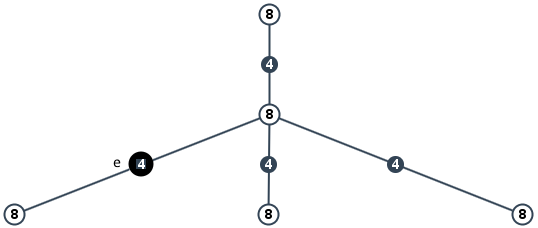
\includegraphics[width=\textwidth]{bilder/abb1_NEU2.png}
				\captionof{figure}{Alle Kanten haben Gewicht 4. Alle Knoten benötigen mindestens 8 Agenten.}
			\end{column}%
			\hfill%
			\begin{column}{.5\textwidth}
				\centering
				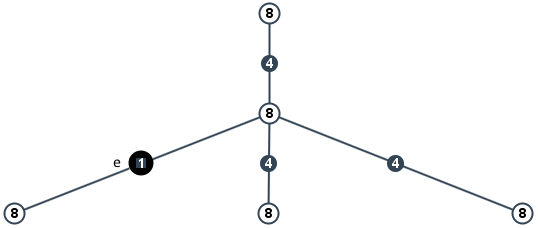
\includegraphics[width=\textwidth]{bilder/abb2_NEU2.png}
				\captionof{figure}{Eine Kante wurde auf Gewicht 1 reduziert, alle anderen Kanten haben weiterhin Gewicht 4. Alle Knoten benötigen trotzdem mindestens 8 Agenten.}
			\end{column}
		\end{columns}

		
	\end{frame}
	
	\begin{frame}
		\frametitle{Das Potential-Problem $k > 1$ auf mehreren Kanten}
		\large
		
		Es gibt Bäume, bei denen das Potential auf linear vielen Kanten verteilt werden muss (hier auf $n-2$):
		
			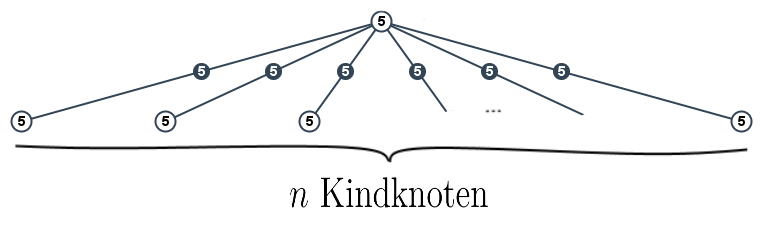
\includegraphics[width=\textwidth]{bilder/abb_bsp_potverteilen.png}
			\captionof{figure}{Die Mindestanzahl an benötigten Kanten kann bei der Potentialverteilung eine Komplexität linear zur Knotenanzahl haben.}
		
	\end{frame}

	\section{Fazit und Aussicht}
	\begin{frame}
		\frametitle{Fazit und Aussicht}
		\large
		
		In dieser Bachelorarbeit war es möglich
		\begin{itemize}
				\item eine Modifikation des Algorithmus zu entwickeln
				\item einen Algorithmus für das Potential-Problem $k = 1$ zu entwickeln
				\item das Potential-Problem $k \geq 1$ auf einer Kante zu lösen
				\item zu Argumentieren, dass es nötig sein kann, das Potential auf mehrere Kanten aufzuteilen
		\end{itemize}
		
	  	 Das Potential-Problem $k > 1$ auf verteilten Kanten konnte im Rahmen dieser Bachelorarbeit nicht gelöst werden, und könnte in Form einer zukünftigen Arbeit weiter untersucht werden.
		
	\end{frame}
	
	\begin{frame}
		\begin{center}
			\large \textbf{Vielen Dank für Ihre Aufmerksamkeit!}
		\end{center}
	\end{frame}

	
	% Literaturliste endgueltig anzeigen
	\begin{frame}
		\frametitle{Quellen}
		\large
		
		\begin{itemize}
			\item Dieser Vortrag basiert auf der Bachelorarbeit "`Optimierung des Intruder-Problems durch Potentialvergabe"'
			
			\item Alle Abbildungen stammen aus dem im Rahmen dieser Bachelorarbeit entwickelten Applet
			
			\item Die Bachelorarbeit basiert auf dem Paper:\\
					\textsc{L. Barrière, P. Flocchini, P. Fraigniaud, N. Santoro} (2002): Capture of an Intruder by Mobile Agents. (SPAA'02) Winnipeg, Manitoba, Canada.
		\end{itemize}
		
	\end{frame}
	
	
%	\begin{thebibliography}{99}
%
%		
%		\bibitem[]{}Alle Abbildungen stammen aus dem im Rahmen dieser Bachelorarbeit entwickelten Applet
%		
%		
%		\bibitem[Ba02]{cima_paper} \textsc{L. Barrière, P. Flocchini, P. Fraigniaud, N. Santoro} (2002): Capture of an Intruder by Mobile Agents. (SPAA'02) Winnipeg, Manitoba, Canada.
%		
%		\bibitem[Fi09]{firefighterproblem_paper} \textsc{S. Finbow, G. MacGillivray} (2009): The Firefighter Problem: A survey of results, directions and questions.
%		AUSTRALASIAN JOURNAL OF COMBINATORICS Vol. 43 (2009), Pages 57–77
%		
%		\bibitem[Kl14]{klein_paper} \textsc{R. Klein, E. Langetepe, C.  Levcopoulos} (2014): A Fire Fighter's Problem. arXiv:1412.6065
%		
%		\bibitem[Me88]{complexity_paper} \textsc{N. Megiddo, S. Hakimi, M. Garey, D. Johnson, C. Papadimitriou} (1988): The Complexity of Searching a Graph. Journal of the ACM, Vol. 35, No 1, 1988.
%		
%		\bibitem[Pa76]{graph_paper_76} \textsc{T. Parson} (1976): Pursuit-evasion problem in a graph. Theory and Applications of Graphs, Lecture Notes in Mathematics, Springer-Verlag, 426-441.
%
%		
%	\end{thebibliography} 

	
\end{document}